\newpage
\section{Exercises: Time-frequency Uncertainty Principle}

\begin{marginfigure}
\begin{center}
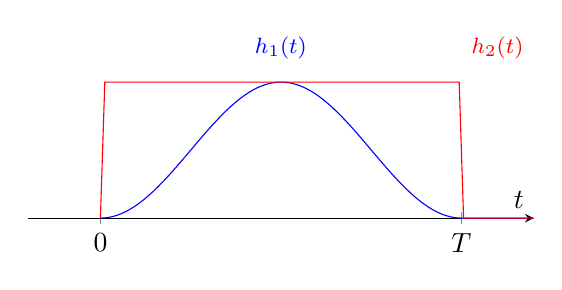
\begin{tikzpicture}
	\begin{axis}[
          width=8cm,
          height=4cm,
          xmin=-0.2,
          xmax=1.2,
          xlabel={$t$},
          ylabel={$h(t)$},
          ymax=1.4,
          ymin=0.0,
          domain=-0.:1.2,
          samples=100,
          axis y line=none,
          axis x line=center, 
          xtick={0,1},
          xticklabels={$0$,$T$}
    ]
          \addplot[blue] {sin(deg(3.14*x))*sin(deg(3.14*x))*(x>0)*(x<1) };
          \node at (axis cs:0.5,1.1) [above, font={\footnotesize}, color=blue]{$h_1(t)$};
          
          \addplot[red] { (x>0)*(x<1) };
          \node at (axis cs:1.1,1.1) [above, font={\footnotesize}, color=red]{$h_2(t)$};          
        \end{axis}
\end{tikzpicture}
\end{center}
\caption{Two impulse responses: 1) a Hann window $h_1(t)$ of length $T$ (blue), and 2) a rectangular window $h_2(t)$ of length $T$ (red).}
\label{fig:hann_ct_ex}
\end{marginfigure}

\begin{marginfigure}
\begin{center}
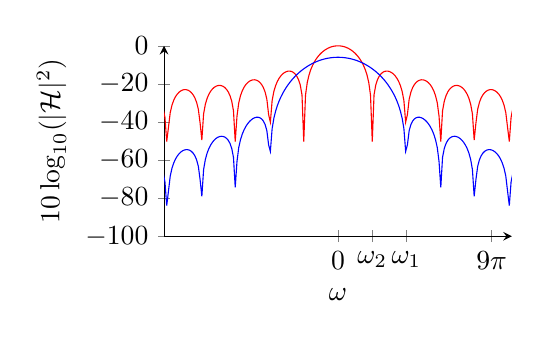
\begin{tikzpicture}
	\begin{axis}[
          width=6cm,
          height=4cm,
          xmin=-32,
          xmax=32,
          xlabel={$\omega$},
          ylabel={$10\log_{10}(|\mathcal{H}|^2)$},
          ymax=0,
          ymin=-100,
          domain=-32.159:32.159,
          samples=200,
          axis y line=left,
          axis x line=bottom, 
          xtick={0,6.28,12.57,28.27},
          xticklabels={$0$,$\omega_2$,$\omega_1$,$9\pi$}
    ]
%          \addplot[blue] {sin(deg(3.14*x))*sin(deg(3.14*x))*(x>0)*(x<1) };
 %         \node at (axis cs:0.5,1.1) [above, font={\footnotesize}, color=blue]{$h_1(t)$};
          
          \addplot[red] { 10.0*log10(abs(2.0*sin(deg(0.5*(x+1e-6)))/(x+1e-6))^2) };
          \addplot[blue] { 10.0*log10(abs(  sin(deg(0.5*(x+1e-6)))/(x+1e-6) + 0.5*(1.0/( (2.0*3.1415) - x ))*sin(deg(3.1415 - 0.5*x)) + 0.5*(1.0/( (2.0*3.1415) + x ))*sin(deg(3.1415 + 0.5*x))        )^2) };          
%          \node at (axis cs:1.1,1.1) [above, font={\footnotesize}, color=red]{$h_2(t)$};          
        \end{axis}
\end{tikzpicture}
\end{center}
\caption{The magnitude responses for the Hann window (blue) and the rectangular window (red). In both cases, the length of the filter is $T=1$. Both are shown in decibel scale.}
\label{fig:hann_ct_ex_mr}
\end{marginfigure}

\begin{enumerate}
\item The Hann window in continuous-time is defined as:
  \begin{equation} h_1(t)= \left\{ \begin{array}{ccc} \sin^2(\pi t/T)
    & \mathrm{when} & 0 \le t \le T \\ 0 & \mathrm{otherwise}
    & \end{array} \right.  \label{eq:hann_h_def_ex} \end{equation}
    Let's define the time-domain width of this filter to be $T$. The
    Hann window is shown in Figure \ref{fig:hann_ct_ex}.

  By using $\sin(\theta) = \frac{1}{2i}(e^{i\theta} - e^{-i\theta})$, it is possible to show that the Fourier transform of the Hann window is:
  \begin{equation}
    \mathcal{H}_1(\omega) = \left[ \frac{\sin(\frac{T}{2}\omega)}{\omega} + \frac{1}{2}\frac{\sin(\pi-\frac{T}{2}\omega)}{\frac{2\pi}{T}-\omega} +  \frac{1}{2}\frac{\sin(\pi+\frac{T}{2}\omega)}{\frac{2\pi}{T}+\omega}  \right] e^{-i\frac{T}{2}\omega}
    \label{eq:hann_ft_result}
  \end{equation}

A rectangular window $h_2(t)$ of length $T$ is also shown in
      Figure \ref{fig:hann_ct_ex}. The Fourier transform of a
      rectangular window of length $T$
      is:
      \begin{equation}
      \mathcal{H}_2(\omega)= \frac{2\sin(\frac{T}{2}\omega)}{\omega}e^{-i \frac{T}{2}\omega}
      \end{equation}      
Both of these filters can be considered to be low pass filters. It is
impossible to unambiguously say that one of these has better frequency
domain properties. The rectangular window has a more narrow pass band
width in frequency domain, while the Hann window has significantly
better rejection of high frequency signals outside the pass
band. Which one you should use will depend on your application.

  \begin{enumerate}[a)]
    \item Show that Equation \ref{eq:hann_ft_result} is the Fourier transform of the signal in Equation \ref{eq:hann_h_def_ex}.
    
    \item The largest value (peak) of the Hann window $h_1(t)$ as
      shown in Figure \ref{fig:hann_ct_ex} is centered at time
      $\frac{T}{2}$. You can easily modify $\mathcal{H}_1(\omega)$ to
      obtain the frequency response of a Hann window, with the peak of
      the impulse response centered at $t=0$ in time. Show how this
      can be done.

    \item Study the magnitude responses for the two filters in decibel
        scale by writing a program to plot 
        $10 \log_{10}(|\mathcal{H}_1(\omega)|^2)$ and
        $10 \log_{10}(|\mathcal{H}_2(\omega)|^2)$. Use the frequency
        range $-10\pi < \omega < 10\pi$ and assume that $T=1$. 

      \item Define the widths of the two filters in frequency domain
        by inspecting the smallest value of $\omega$ for which
        $| \mathcal{H}(\omega)|=0$, i.e., the first null of the
        magnitude response. You can also use
        Figure \ref{fig:hann_ct_ex_mr} to help you out. In the case of
        $\mathcal{H}_2(\omega)$, the first null is at $\omega_2 =
        2\pi/T$ and the null-to-null width of the rectangular filter is
        thus $\Delta \omega_2 = 2\omega_2 = 4\pi/T$. From
        Figure \ref{fig:hann_ct_ex_mr}, it appears that the
        null-to-null width of the Hann filter in frequency domain is
        twice that of the rectangular window $\Delta \omega_1 =
        2\Delta \omega_2$. Show that this is the case\sidenote{Note that the width of the passband of a frequency symmetric low-pass filter in frequency domain is often given in terms of half-power width, not null-to-null width. In most cases, this needs to be numerically evaluated, so we haven't done this here. The half-power width is defined based on the following property:
        \begin{equation}
        |\mathcal{H}(\omega')|^2 = \frac{1}{2} |\mathcal{H}(0)|^2
        \end{equation}
        with the half-power width being $\Delta\omega_{1/2}=2\omega'$. }.
        

        \item How long do the two filters need (in seconds) to be in
        order to achieve a null-to-null pass bandwidth of
        $\Delta \omega = 2\pi$ rad/s?



\item Recall that if a complex sinusoidal signal
    \begin{equation}
    x(t) = e^{i\omega' t}
    \end{equation}
    is fed into an LTI system with impulse response $h(t)$, the output signal would be of the form:
    \begin{equation}
    y(t) = |\mathcal{H}(\omega')|e^{i\angle \mathcal{H}(\omega')}e^{i\omega' t}
    \end{equation}
    
    Assuming that $T=1$ s and $\omega'=9\pi$ rad/s, what would the
    amplitudes of the complex sinusoidal signals coming out of the 
    Hann and rectangular filters ($|\mathcal{H}_1(9\pi)|$ and
    $|\mathcal{H}_2(9\pi)|$) be? You don't necessarily need to obtain an
    exact number, you can look at Figure \ref{fig:hann_ct_ex_mr} and
    estimate it from there.

    \item While the rectangular filter has a more narrow filter width
    in frequency domain than a Hann window of the same length, the
    Hann window is in most cases significantly better when it comes to
    filtering out frequency components with frequencies outside
    the passband. Explain why by comparing the magnitude responses of
    the rectangular and Hann windows in decibel scale, shown in
    Figure \ref{fig:hann_ct_ex_mr}.
            

      
  \end{enumerate}


\item Consider the following function:
\begin{equation}
\Psi(x) = \frac{1}{\sqrt{2T}}[u(x + T) - u(x - T)].
\end{equation}
The function $|\Psi(x)|^{2}$ describes the probability density of
finding a particle at position $x$.

\begin{enumerate}[a)]
\item Show that:
\begin{align*}
\hat{\Psi}(k)&= \frac{1}{\sqrt{2\pi}}\int_{-\infty}^{\infty}\Psi(x)e^{-ik x}dx, \\
            &= \frac{1}{\sqrt{T\pi}}\frac{\sin(k T)}{k}.
\end{align*}
Here $\hat{\Psi}(k)$ is the unitary Fourier transform\sidenote[][-3cm]{The
unitary Fourier transform pair is defined
as:\begin{align*}
\hat{f}(\omega)&=\frac{1}{\sqrt{2\pi}}\int_{-\infty}^{\infty}
f(t) e^{-i\omega t}dt \\
f(t) &=\frac{1}{\sqrt{2\pi}}\int_{-\infty}^{\infty} \hat{f}(\omega)
e^{i\omega t}d\omega
\end{align*}
This version of the Fourier transform results in the following variant of Plancherel's theorem:
\begin{equation*}
\int_{-\infty}^{\infty} \hat{f}(\omega)\hat{g}^*(\omega) d\omega = \int_{-\infty}^{\infty} f(t)g^*(t) dt.
\end{equation*}
This theorem was derived in the Fourier transform chapter (see Equation \ref{eq:ft_plancherel_theorem}).

} of $\Psi(x)$. The function $|\hat{\Psi}(k)|^{2}$ is the probability
density function for the particle having the wavenumber $k$. If $x$
has units of meters, then $k$ has units of rad/m. In this case, the
particle momentum and wavenumber are related as follows:
$p = \hbar k$ with units of kg$\cdot$m$/$s.

\item Define the width of the wave functions $\Psi(x)$ and $\hat{\Psi}(k)$.
\footnote{A solution to the Schrödinger equation is called a wave function. If you aren't familiar with quantum mechanics, just think of it as an ordinary function.} 
We'll define the width of the wavefunctions in the following way:
$$\Delta x = \min\{x : |\Psi(x)|^{2}=0,x>0\},$$
and 
$$\Delta k = \min\{k : |\hat{\Psi}(k)|^{2}=0,k>0\},$$
or, in other words, $\Delta x$ and $\Delta k$ are the smallest positive values for which the functions $|\Psi(x)|^{2}$ and $|\hat{\Psi}(k)|^{2}$ are $0$. 
Determine $\Delta x$ and $\Delta k$ for the functions $\Psi(x)$ and $\hat{\Psi}(k)$ and come up with a relation between $\Delta x$ and $\Delta k$.

\item Sketch the functions $\Psi(x)$ and $\hat{\Psi}(k)$ and indicate $\Delta x$ and $\Delta k$ in your drawing. 

\item Show that:
$$\int_{-\infty}^{\infty} |\hat{\Psi}(k)|^{2}dk=1.$$ The meaning of this
integral is that we are 100\% certain that a particle will have a wavenumber in the range $-\infty<k<\infty$.

\item Now consider another wavefunction that describes the position of a particle:
\begin{equation}
\Psi(x) = \delta(x-x_0),
\end{equation}
where $x_0$ is the position of the particle. Can you say that one
value of momentum or wavenumber is more probable than another?

\end{enumerate}



\end{enumerate}
